\documentclass[tikz]{standalone}

\usepackage{tikz}
\usetikzlibrary{positioning,arrows,shapes}

\begin{document}
  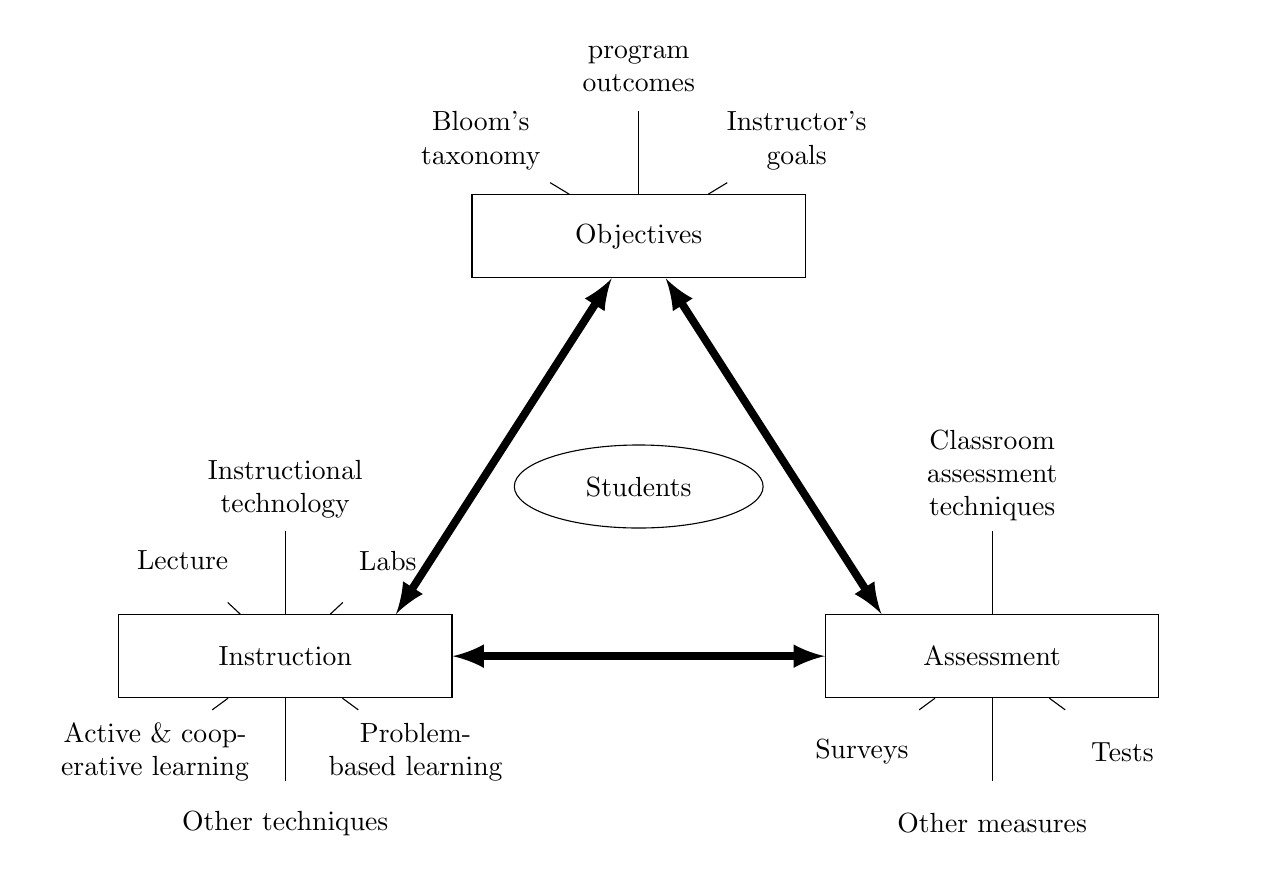
\begin{tikzpicture}[node distance = 1em, auto,
    dimension/.style={draw, rectangle, text width=4cm, align=center, minimum height=3em},
    component/.style={text width=3cm, align=center, minimum height=3em}
    ]
    \node[draw, ellipse, minimum size=30pt, text width=2cm, align=center] (students) at (0,0) {Students};
    \node[dimension, above=6em of students] (objectives) {Objectives};
    \node[dimension, below left=5em of students] (instruction) {Instruction};
    \node[dimension, below right=5em of students] (assessment) {Assessment};
    \draw[<->,>=latex,line width=1mm] ([xshift=4em]instruction.north) to (objectives);
    \draw[<->,>=latex,line width=1mm] (objectives) to ([xshift=-4em]assessment.north);
    \draw[<->,>=latex,line width=1mm] (instruction) to (assessment);

    \node[component, above=3em of objectives] (program_outcomes) {program\\ outcomes};
    \node[below left=of program_outcomes] (o1) {};
    \node[component, right=-5em of o1] (blooms) {Bloom's\\ taxonomy};
    \node[below right=of program_outcomes] (o2) {};
    \node[component, left=-5em of o2] (instructor_goals) {Instructor's\\ goals};
    
    \foreach \component in {blooms,program_outcomes,instructor_goals} {
      \draw[] (\component) to (objectives);
    };
    
    \node[component, above=3em of instruction] (IT) {Instructional technology};
    \node[below left=of IT] (i1) {};
    \node[component, right=-3em of i1] (lecture) {Lecture};
    \node[below right=of IT] (i2) {};
    \node[component, left=-3em of i2] (labs) {Labs};
    
    \node[component, below=3em of instruction] (other_instruction) {Other techniques};
    \node[above left=of other_instruction] (i3) {};
    \node[component, right=-4em of i3] (active) {Active \& cooperative learning};
    \node[above right=of other_instruction] (i4) {};
    \node[component, left=-4em of i4](PBL) {Problem-based learning};
    
    \foreach \component in {lecture,labs,other_instruction,active,PBL,IT} {
      \draw[] (\component) to (instruction);
    };
    
    \node[component, below=3em of assessment] (other_measures) {Other measures};
    \node[above left=of other_measures] (a1) {};
    \node[component, right=-4em of a1] (surveys) {Surveys};
    \node[above right=of other_measures] (a2) {};
    \node[component, left=-4em of a2] (tests) {Tests};
    \node[component, above=3em of assessment] (CATs) {Classroom assessment techniques};
    
    \foreach \component in {CATs,surveys,other_measures,tests} {
      \draw[] (\component) to (assessment);
    };
  \end{tikzpicture}  
\end{document}
